% Options for packages loaded elsewhere
\PassOptionsToPackage{unicode}{hyperref}
\PassOptionsToPackage{hyphens}{url}
\PassOptionsToPackage{dvipsnames,svgnames,x11names}{xcolor}
%
\documentclass[
  letterpaper,
  DIV=11,
  numbers=noendperiod]{scrreprt}

\usepackage{amsmath,amssymb}
\usepackage{lmodern}
\usepackage{iftex}
\ifPDFTeX
  \usepackage[T1]{fontenc}
  \usepackage[utf8]{inputenc}
  \usepackage{textcomp} % provide euro and other symbols
\else % if luatex or xetex
  \usepackage{unicode-math}
  \defaultfontfeatures{Scale=MatchLowercase}
  \defaultfontfeatures[\rmfamily]{Ligatures=TeX,Scale=1}
\fi
% Use upquote if available, for straight quotes in verbatim environments
\IfFileExists{upquote.sty}{\usepackage{upquote}}{}
\IfFileExists{microtype.sty}{% use microtype if available
  \usepackage[]{microtype}
  \UseMicrotypeSet[protrusion]{basicmath} % disable protrusion for tt fonts
}{}
\makeatletter
\@ifundefined{KOMAClassName}{% if non-KOMA class
  \IfFileExists{parskip.sty}{%
    \usepackage{parskip}
  }{% else
    \setlength{\parindent}{0pt}
    \setlength{\parskip}{6pt plus 2pt minus 1pt}}
}{% if KOMA class
  \KOMAoptions{parskip=half}}
\makeatother
\usepackage{xcolor}
\setlength{\emergencystretch}{3em} % prevent overfull lines
\setcounter{secnumdepth}{-\maxdimen} % remove section numbering
% Make \paragraph and \subparagraph free-standing
\ifx\paragraph\undefined\else
  \let\oldparagraph\paragraph
  \renewcommand{\paragraph}[1]{\oldparagraph{#1}\mbox{}}
\fi
\ifx\subparagraph\undefined\else
  \let\oldsubparagraph\subparagraph
  \renewcommand{\subparagraph}[1]{\oldsubparagraph{#1}\mbox{}}
\fi

\usepackage{color}
\usepackage{fancyvrb}
\newcommand{\VerbBar}{|}
\newcommand{\VERB}{\Verb[commandchars=\\\{\}]}
\DefineVerbatimEnvironment{Highlighting}{Verbatim}{commandchars=\\\{\}}
% Add ',fontsize=\small' for more characters per line
\usepackage{framed}
\definecolor{shadecolor}{RGB}{241,243,245}
\newenvironment{Shaded}{\begin{snugshade}}{\end{snugshade}}
\newcommand{\AlertTok}[1]{\textcolor[rgb]{0.68,0.00,0.00}{#1}}
\newcommand{\AnnotationTok}[1]{\textcolor[rgb]{0.37,0.37,0.37}{#1}}
\newcommand{\AttributeTok}[1]{\textcolor[rgb]{0.40,0.45,0.13}{#1}}
\newcommand{\BaseNTok}[1]{\textcolor[rgb]{0.68,0.00,0.00}{#1}}
\newcommand{\BuiltInTok}[1]{\textcolor[rgb]{0.00,0.23,0.31}{#1}}
\newcommand{\CharTok}[1]{\textcolor[rgb]{0.13,0.47,0.30}{#1}}
\newcommand{\CommentTok}[1]{\textcolor[rgb]{0.37,0.37,0.37}{#1}}
\newcommand{\CommentVarTok}[1]{\textcolor[rgb]{0.37,0.37,0.37}{\textit{#1}}}
\newcommand{\ConstantTok}[1]{\textcolor[rgb]{0.56,0.35,0.01}{#1}}
\newcommand{\ControlFlowTok}[1]{\textcolor[rgb]{0.00,0.23,0.31}{#1}}
\newcommand{\DataTypeTok}[1]{\textcolor[rgb]{0.68,0.00,0.00}{#1}}
\newcommand{\DecValTok}[1]{\textcolor[rgb]{0.68,0.00,0.00}{#1}}
\newcommand{\DocumentationTok}[1]{\textcolor[rgb]{0.37,0.37,0.37}{\textit{#1}}}
\newcommand{\ErrorTok}[1]{\textcolor[rgb]{0.68,0.00,0.00}{#1}}
\newcommand{\ExtensionTok}[1]{\textcolor[rgb]{0.00,0.23,0.31}{#1}}
\newcommand{\FloatTok}[1]{\textcolor[rgb]{0.68,0.00,0.00}{#1}}
\newcommand{\FunctionTok}[1]{\textcolor[rgb]{0.28,0.35,0.67}{#1}}
\newcommand{\ImportTok}[1]{\textcolor[rgb]{0.00,0.46,0.62}{#1}}
\newcommand{\InformationTok}[1]{\textcolor[rgb]{0.37,0.37,0.37}{#1}}
\newcommand{\KeywordTok}[1]{\textcolor[rgb]{0.00,0.23,0.31}{#1}}
\newcommand{\NormalTok}[1]{\textcolor[rgb]{0.00,0.23,0.31}{#1}}
\newcommand{\OperatorTok}[1]{\textcolor[rgb]{0.37,0.37,0.37}{#1}}
\newcommand{\OtherTok}[1]{\textcolor[rgb]{0.00,0.23,0.31}{#1}}
\newcommand{\PreprocessorTok}[1]{\textcolor[rgb]{0.68,0.00,0.00}{#1}}
\newcommand{\RegionMarkerTok}[1]{\textcolor[rgb]{0.00,0.23,0.31}{#1}}
\newcommand{\SpecialCharTok}[1]{\textcolor[rgb]{0.37,0.37,0.37}{#1}}
\newcommand{\SpecialStringTok}[1]{\textcolor[rgb]{0.13,0.47,0.30}{#1}}
\newcommand{\StringTok}[1]{\textcolor[rgb]{0.13,0.47,0.30}{#1}}
\newcommand{\VariableTok}[1]{\textcolor[rgb]{0.07,0.07,0.07}{#1}}
\newcommand{\VerbatimStringTok}[1]{\textcolor[rgb]{0.13,0.47,0.30}{#1}}
\newcommand{\WarningTok}[1]{\textcolor[rgb]{0.37,0.37,0.37}{\textit{#1}}}

\providecommand{\tightlist}{%
  \setlength{\itemsep}{0pt}\setlength{\parskip}{0pt}}\usepackage{longtable,booktabs,array}
\usepackage{calc} % for calculating minipage widths
% Correct order of tables after \paragraph or \subparagraph
\usepackage{etoolbox}
\makeatletter
\patchcmd\longtable{\par}{\if@noskipsec\mbox{}\fi\par}{}{}
\makeatother
% Allow footnotes in longtable head/foot
\IfFileExists{footnotehyper.sty}{\usepackage{footnotehyper}}{\usepackage{footnote}}
\makesavenoteenv{longtable}
\usepackage{graphicx}
\makeatletter
\def\maxwidth{\ifdim\Gin@nat@width>\linewidth\linewidth\else\Gin@nat@width\fi}
\def\maxheight{\ifdim\Gin@nat@height>\textheight\textheight\else\Gin@nat@height\fi}
\makeatother
% Scale images if necessary, so that they will not overflow the page
% margins by default, and it is still possible to overwrite the defaults
% using explicit options in \includegraphics[width, height, ...]{}
\setkeys{Gin}{width=\maxwidth,height=\maxheight,keepaspectratio}
% Set default figure placement to htbp
\makeatletter
\def\fps@figure{htbp}
\makeatother
\newlength{\cslhangindent}
\setlength{\cslhangindent}{1.5em}
\newlength{\csllabelwidth}
\setlength{\csllabelwidth}{3em}
\newlength{\cslentryspacingunit} % times entry-spacing
\setlength{\cslentryspacingunit}{\parskip}
\newenvironment{CSLReferences}[2] % #1 hanging-ident, #2 entry spacing
 {% don't indent paragraphs
  \setlength{\parindent}{0pt}
  % turn on hanging indent if param 1 is 1
  \ifodd #1
  \let\oldpar\par
  \def\par{\hangindent=\cslhangindent\oldpar}
  \fi
  % set entry spacing
  \setlength{\parskip}{#2\cslentryspacingunit}
 }%
 {}
\usepackage{calc}
\newcommand{\CSLBlock}[1]{#1\hfill\break}
\newcommand{\CSLLeftMargin}[1]{\parbox[t]{\csllabelwidth}{#1}}
\newcommand{\CSLRightInline}[1]{\parbox[t]{\linewidth - \csllabelwidth}{#1}\break}
\newcommand{\CSLIndent}[1]{\hspace{\cslhangindent}#1}

\usepackage{amsmath}
\usepackage{booktabs}
\usepackage{caption}
\usepackage{longtable}
\KOMAoption{captions}{tableheading}
\makeatletter
\makeatother
\makeatletter
\@ifpackageloaded{bookmark}{}{\usepackage{bookmark}}
\makeatother
\makeatletter
\@ifpackageloaded{caption}{}{\usepackage{caption}}
\AtBeginDocument{%
\ifdefined\contentsname
  \renewcommand*\contentsname{Table of contents}
\else
  \newcommand\contentsname{Table of contents}
\fi
\ifdefined\listfigurename
  \renewcommand*\listfigurename{List of Figures}
\else
  \newcommand\listfigurename{List of Figures}
\fi
\ifdefined\listtablename
  \renewcommand*\listtablename{List of Tables}
\else
  \newcommand\listtablename{List of Tables}
\fi
\ifdefined\figurename
  \renewcommand*\figurename{Figur}
\else
  \newcommand\figurename{Figur}
\fi
\ifdefined\tablename
  \renewcommand*\tablename{Tabell}
\else
  \newcommand\tablename{Tabell}
\fi
}
\@ifpackageloaded{float}{}{\usepackage{float}}
\floatstyle{ruled}
\@ifundefined{c@chapter}{\newfloat{codelisting}{h}{lop}}{\newfloat{codelisting}{h}{lop}[chapter]}
\floatname{codelisting}{Listing}
\newcommand*\listoflistings{\listof{codelisting}{List of Listings}}
\makeatother
\makeatletter
\@ifpackageloaded{caption}{}{\usepackage{caption}}
\@ifpackageloaded{subcaption}{}{\usepackage{subcaption}}
\makeatother
\makeatletter
\@ifpackageloaded{tcolorbox}{}{\usepackage[many]{tcolorbox}}
\makeatother
\makeatletter
\@ifundefined{shadecolor}{\definecolor{shadecolor}{rgb}{.97, .97, .97}}
\makeatother
\makeatletter
\makeatother
\ifLuaTeX
  \usepackage{selnolig}  % disable illegal ligatures
\fi
\IfFileExists{bookmark.sty}{\usepackage{bookmark}}{\usepackage{hyperref}}
\IfFileExists{xurl.sty}{\usepackage{xurl}}{} % add URL line breaks if available
\urlstyle{same} % disable monospaced font for URLs
\hypersetup{
  pdftitle={Deloppgave 4 Study Designs},
  pdfauthor={INGER JOHANNE LØKKEVIK},
  colorlinks=true,
  linkcolor={blue},
  filecolor={Maroon},
  citecolor={Blue},
  urlcolor={Blue},
  pdfcreator={LaTeX via pandoc}}

\title{Deloppgave 4 Study Designs}
\author{INGER JOHANNE LØKKEVIK}
\date{2022-11-22}

\begin{document}
\maketitle
\ifdefined\Shaded\renewenvironment{Shaded}{\begin{tcolorbox}[sharp corners, enhanced, frame hidden, borderline west={3pt}{0pt}{shadecolor}, interior hidden, boxrule=0pt, breakable]}{\end{tcolorbox}}\fi

\renewcommand*\contentsname{Table of contents}
{
\hypersetup{linkcolor=}
\setcounter{tocdepth}{2}
\tableofcontents
}
\bookmarksetup{startatroot}

\hypertarget{preface}{%
\chapter*{Preface}\label{preface}}
\addcontentsline{toc}{chapter}{Preface}

\markboth{Preface}{Preface}

This is a Quarto book.

To learn more about Quarto books visit
\url{https://quarto.org/docs/books}.

\begin{Shaded}
\begin{Highlighting}[]
\DecValTok{1} \SpecialCharTok{+} \DecValTok{1}
\end{Highlighting}
\end{Shaded}

\begin{verbatim}
[1] 2
\end{verbatim}

\bookmarksetup{startatroot}

\hypertarget{deloppgave-1-beskrivende-statistikk-reliabilitet-og-validitet-verktuxf8y-for-reproduserbar-dataanalyse}{%
\chapter{Deloppgave 1: Beskrivende statistikk, reliabilitet og
validitet, verktøy for reproduserbar
dataanalyse}\label{deloppgave-1-beskrivende-statistikk-reliabilitet-og-validitet-verktuxf8y-for-reproduserbar-dataanalyse}}

\bookmarksetup{startatroot}

\hypertarget{introduksjon-og-metode}{%
\chapter{Introduksjon og metode}\label{introduksjon-og-metode}}

\hypertarget{laktatprofil-luxf8p}{%
\subsection{Laktatprofil løp}\label{laktatprofil-luxf8p}}

Vi har gjennomført laktattesting av til sammen 7 masterstudenter i
aldersgruppen 23-50 år i løping på tredemølle. Det er gjennomført to
tester (Pre og Post) av alle, men det er ikke gjennomført intervensjon i
perioden mellom testene. Testen ble gjennomført som en laktatprofil med
en standarisert trappetrinnsprotokoll der farten økte med 1,5km/t per
drag til forsøkspersonen passerte en laktatkonsentrasjon høyere enn
4mmol/L. Grunnet tekniske utfordringer, ble testprotokollen
(fartsøkningsintervallet) endret etter testing av to individer. Disse to
er imidlertid testet likt begge ganger selv om hastighetene ikke var lik
på alle trappetrinn som resten av gruppen.

Det er tilstrebet å redusere antall ytre faktorer som kan påvirke
testresultatene gjennom å standardisere forberedelser av testpersonene
og testsituasjonen.

Utstyr benyttet til analyse har vært det samme gjennom all testing, og
er kalibrert mellom hver test. Bionsen er benyttet for analyse av laktat
og Jaeger Oxycon Pro analyserer ventilasjon, puls, O2 forbruk.

Det er kjent at hydrerings- og ernæringtilstand påvirker testresultater.
Redusert energitilgjengelighet (\textless30 kcal /kg fettfri masse/dag)
forventes å påvirke metabolismen og prestasjon negativt. Inntak av
karbohydrat i forkant av og under test, medfører økt glykogen
tilgjengelighet. Lavt inntak kan medføre hypoglykemi og dårligere
prestasjon. Koffeininntak i forkant av test har vist økt prestasjon, men
hvis man er vant til å innta koffein daglig, bør dette også gjøres
testdag, da abstinenser kan medføre hodepine og tretthet. Alkoholinntak
kan påvirke hydreringstilstand og karbohydratmetabolismen og derved gi
redusert prestasjon (Tanner \& Gore, 2012).

Testpersonene i undersøkelsen er derfor forberedt og instruert i å
trene, spise og sove likt før testene. Testutstyr som sko og tøy har
også vært det samme under testing.

Ut over forberedelse av testperson, er det forhold ved testsituasjonen
som kan påvirke resultatet. Temperatur og luftfuktighet bør tilstrebes å
være lik under all testing. Andre kjente faktorer som kan påvirke
testresultater er testpersonens kjennskap til testforløpet,
tilbakemeldinger testpersonen får underveis, antall testpersoner i
lokalet og kjønnsfordeling på disse, ``dagsform'' eller mentalt
overskudd hos testpersonen og om testpersonen hører musikk før og under
testing (Halperin, Pyne, and Martin 2015).

Testing er derfor tilstrebet gjennomført med: Testtidspunkt samme tid på
døgnet. Samme testleder på pre og post test. Samme antall og kjønn
tilstede ved alle tester. Ingen musikk før/under test. Tilnærmet lik
tilbakemelding og engasjement fra testleder. Det er opplyst om videre
hendelsesforløp før hver endring (forklart test, tempoøkninger, tid
igjen osv.) Det er ikke opplyst om puls, laktat og VO2. Notert ned evt.
når og hvor mye forsøkspersonen drikker/spiser og repetert ved post-test

Møllen har vært innstilt på 1 \% stigning, og det er kjørt 5 minutters
drag med 1 minutts pause. Utgangshastighet var på 8,5 km/t, og denne ble
økt med 1,5km/t per drag til FP målte over 4 mmol/L Lac.

Under testing, er data samlet inn via analysemaskin for laktat (Bionsen)
og Jaeger Oxycon Pro, som analyserer ventilasjon, puls, O2 forbruk. Data
er hentet ut i etterkant. Innsamlede data er i tillegg sikret løpende
manuelt i plotteskjema. Alle data er etterfølgende lagt inn i et
excelark (Data\_run\_2) før videre analyse.

\bookmarksetup{startatroot}

\hypertarget{statistikk}{%
\chapter{Statistikk}\label{statistikk}}

Statistisk analyse er utført i RStudio 2022.07.2. Det er beregnet mean,
median, standardavvik og varians av maksimale verdier pre og post. Det
er beregnet standardavvik, typical error, og variasjonskoeffesient av
differansen.

\bookmarksetup{startatroot}

\hypertarget{deskriptive-data}{%
\chapter{Deskriptive data}\label{deskriptive-data}}

\begin{verbatim}
Rows: 14
Columns: 12
$ FP         <dbl> 1, 1, 2, 2, 3, 3, 4, 4, 5, 5, 6, 6, 7, 7
$ Gender     <chr> "Male", "Male", "Female", "Female", "Male", "Male", "Male",~
$ Timepoint  <chr> "Pre", "Post", "Pre", "Post", "Pre", "Post", "Pre", "Post",~
$ Age        <dbl> 24, 24, 50, 50, 23, 23, 29, 29, 25, 25, 23, 23, 23, 23
$ Height     <dbl> 195, 195, 169, 169, 175, 175, 180, 180, 191, 191, 171, 171,~
$ Weigth     <dbl> 86.0, 86.0, 56.1, 56.1, 81.9, 81.9, 93.4, 93.1, 80.7, 79.9,~
$ start.load <dbl> 10.0, 13.0, 8.5, 8.5, 8.5, 8.5, 12.0, 10.0, 8.5, 8.5, 8.5, ~
$ end.load   <dbl> 19.0, 19.0, 11.5, 11.5, 16.0, 14.5, 15.0, 15.0, 14.5, 14.5,~
$ VO2.max    <dbl> 5293, 5224, 2239, 2290, 4525, 3937, 4527, 4613, 4179, 4201,~
$ lac.max    <dbl> 8.31, 5.33, 5.68, 5.20, 6.14, 5.00, 4.47, 4.12, 7.45, 5.41,~
$ HR.max     <chr> "196", "201", "168", "169", "182", "180", "180", "175", "NA~
$ RER.max    <dbl> 1.00, 1.01, 0.99, 0.96, 1.01, 1.03, 0.96, 0.99, 1.10, 1.20,~
\end{verbatim}

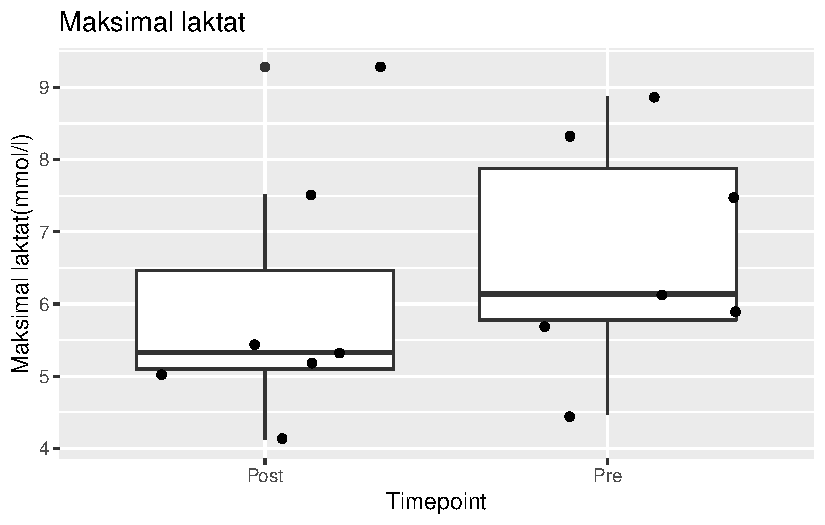
\includegraphics{./part1_files/figure-pdf/unnamed-chunk-2-1.pdf}

\bookmarksetup{startatroot}

\hypertarget{resultater}{%
\chapter{Resultater}\label{resultater}}

\begin{longtable}{lrrrr}
\caption*{
{\large Gjennomsnittlige maksimale verdier}
} \\ 
\toprule
Test & Max Laktat & Max RER & VO2max(ml min-1) & Max fart(km t-1) \\ 
\midrule
Post & $5.98$ & $1.05$ & $3,780$ & $13.9$ \\ 
Pre & $6.69$ & $1.01$ & $3,822$ & $14.1$ \\ 
\bottomrule
\end{longtable}

\setlength{\LTpost}{0mm}
\begin{longtable}{lrrrr}
\caption*{
{\large Medianverdier}
} \\ 
\toprule
Test & Max Laktat & Max RER & VO2max(ml min-1) & Max fart(km t-1) \\ 
\midrule
Post & $5.33$ & $1.03$ & $3,937$ & $13.9$ \\ 
Pre & $6.14$ & $1.00$ & $4,179$ & $14.1$ \\ 
\bottomrule
\end{longtable}
\begin{minipage}{\linewidth}
median av maksimale verdier\\
\end{minipage}

\setlength{\LTpost}{0mm}
\begin{longtable}{lrrrr}
\caption*{
{\large Standardavvik}
} \\ 
\toprule
Test & Max Laktat & Max RER & VO2max(ml min-1) & Max fart(km t-1) \\ 
\midrule
Post & $1.78$ & $0.08$ & $1,025$ & $2.8$ \\ 
Pre & $1.58$ & $0.04$ & $1,095$ & $2.9$ \\ 
\bottomrule
\end{longtable}
\begin{minipage}{\linewidth}
SD av maksimale verdier\\
\end{minipage}

\begin{longtable}{lrrrr}
\caption*{
{\large VARIANS}
} \\ 
\toprule
Test & Max Laktat & Max RER & VO2max(ml min-1) & Max fart(km t-1) \\ 
\midrule
Post & $3.17$ & $0.01$ & $1,049,849$ & $8.0$ \\ 
Pre & $2.48$ & $0.00$ & $1,198,619$ & $8.6$ \\ 
\bottomrule
\end{longtable}

\begin{verbatim}
# A tibble: 1 x 4
     sd    te     m    cv
  <dbl> <dbl> <dbl> <dbl>
1  1.53  1.08  6.33  17.1
\end{verbatim}

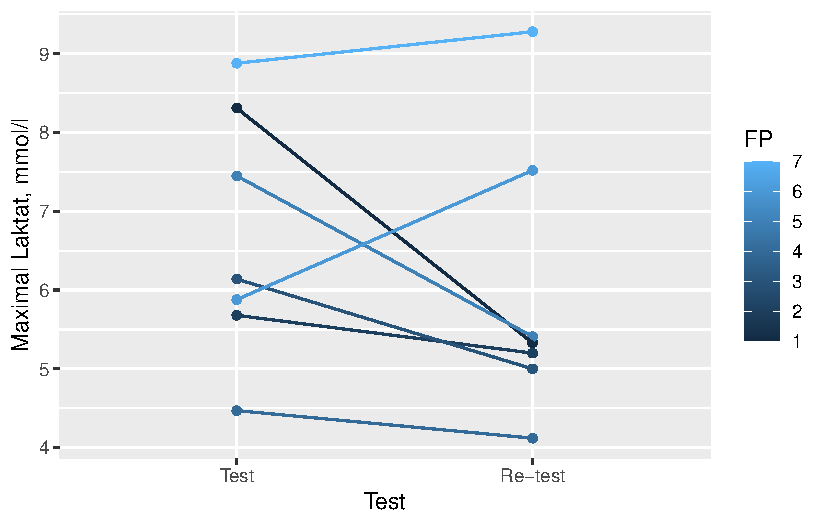
\includegraphics{./part1_files/figure-pdf/unnamed-chunk-8-1.pdf}

\bookmarksetup{startatroot}

\hypertarget{konklusjon}{%
\chapter{Konklusjon}\label{konklusjon}}

Vi har valgt å gjøre beregninger ut fra høyeste målte laktat pr test.
Test ble ikke gjennomført helt i henhold til protokoll, grunnet tidsnød
i lab. Flere av forsøkspersonene ble testet rett hverandre, med kun 10
minutter mellom testene. Protokollen ble endret underveis, og selv om
dette ikke skal påvirke forholdet mellom pre- og post-testingen er det
en svakhet ved forsøket. Konstant utskiftning av testpersonell også en
sentral faktor til feilkilde. Når testene utføres av forskjellig
testpersonell vil dette kunne gi utslag på resultatene, og være en
feilkilde for spesielt ``within-subject variation'' (Hopkins 2000).
Eksempelvis vil resultatet på laktatprøvene avhenge av hvordan testeren
tar selve prøven, hvor lang tid som brukes, og om prøven utføres
korrekt. I vårt forsøk er Typical Error (TE) beregnet til 1,08. Typical
Error vil indikere forskjellen i avviket fra gjennomsnittet i to
gruppene. Standardavvik (sd) er beregnet til 1,53 og
varasjonskoeffisient (cv) til 17\%. Standardavviket er avviket fra
gjennomsnittet. Variasjonskoeffesienten kan beskrives som
standardavviket i forhold til gjennomsnittet i prosent. 17\% anses som
en stor variasjon, noe som tyder på lav reliabilitet.

\bookmarksetup{startatroot}

\hypertarget{referanser}{%
\chapter{Referanser}\label{referanser}}

Tanner, R. K., and C. J. Gore. 2012. Physiological Tests for Elite
Athletes 2nd Edition. Book. Human Kinetics.
https://books.google.no/books?id=0OPIiMks58MC

\begin{center}\rule{0.5\linewidth}{0.5pt}\end{center}

\bookmarksetup{startatroot}

\hypertarget{deloppgave-2-labrapport}{%
\chapter{Deloppgave 2: LABRAPPORT}\label{deloppgave-2-labrapport}}

\textless--- title: ``Labrapport: Ekstraksjon og analyse av DNA''
author: ``Pia Julie Demler, Emil Hosøy, Emil Åberg, Inger Johanne
Løkkevik'' format: html editor: visual bibliography: references.bib ---

\hypertarget{introduksjon}{%
\section{\texorpdfstring{\textbf{Introduksjon}}{Introduksjon}}\label{introduksjon}}

Fysisk prestasjon påvirkes av mange forskjellige faktorer. Et fokus de
siste årene har vært forskning på genetikks påvirkning på prestasjon. Et
gen som ofte er assosiert med muskelfunksjon og fysisk prestasjonsevne
er ACTN3 (Pickering and Kiely 2017). ACTN3 står for alfa-actinin-3 og
koder for et protein som kun finnes i type-II muskelfibre. Proteinet er
involvert i muskelkontraksjon og bidrar til å skape eksplosiv kraft ved
høye hastigheter (Yang et al. 2003). En polymorfisme av genet er R577X.
Her erstattes arginin (R) med et prematurt stoppkodon (X) ved aminosyre
577, noe som resulterer i en forkortet versjon av genet (Eynon et al.
2012). R-allelen er assosiert med kraftidretter og X-allelen finnes for
det meste hos utholdenhetsutøvere.

En metode som ofte brukes for å bestemme denne polymorfismen er
RFLP-teknikken (restriction fragment length polymorphism technique) og
real-time polymerasekjedereaksjon (PCR). En enklere og billigere metode
er presentert av Schadock et al. (2015): her utføres en enkelt PCR-test
med 4 primere. Resultatene ble validert ved hjelp av real-time
PCR-metoden. Schadock et al. (2015) bruker primere som viser et produkt
ved henholdsvis 413 basepar og 318 basepar når en R- eller X-allel er
til stede.

I denne undersøkelsen ble DNA ekstrahert fra helblod, etter videre
bearbeiding og gjennomføring av PCR-test ble genotypene bestemt ved
hjelp av gelelektroforese.

\hypertarget{metode}{%
\section{\texorpdfstring{\textbf{Metode}}{Metode}}\label{metode}}

Fra helblod har vi ekstrahert DNA i henhold til protokoll adaptert fra
Bartlett \& Stirling (2003). Dette har vi brukt til å bestemme ACTN3
genotype ved hjelp av protokoll adaptert fra Schadock et al. (2015).

Det ble innhentet blod i EDTA-rør fra hver av deltakerne ( P, IJ, EÅ, og
EH). 3 mL blod ble pipettert over i et 15 mL rør. Vortex før
pipettering. Deretter tilsatte vi 12 mL reagens A. Dette ble mixet ved
rotasjon i 4 minutter. Deretter sentrifugerte vi rørene ved 3000g i 5
min ved romtemperatur. Supernatanten avpipetteres og kastes uten at
cellepellets forstyrres. All overskuddsvæske fjernes. Reagens B
tilsettes før vortex 30s.

250 µL 5M natriumperklorat ble tilsatt og det hele ble blandet ved rolig
vending av røret før det ble plassert i vannbad (65°C) i 15-20 min.
Prøven ble deretter avkjølt til romtemperatur og tilsatt 2 mL iskald
kloroform, blandet på roterende mikser i 60 minutter, og sentrifugert
ved 2400g i 2 min.

Den øvre fasen ble deretter avpipettert over i et rent falcon-rør med en
steril pipette. Ved å tilsette 2 mL avkjølt 100\% etanol, utfelles DNA.
Dette overførte vi til et 1.5 mL rør og fjernet overskuddsvæske før vi
lot DNA'et lufttørke. Vi tilførte deretter 200µL av TE bufferen. For å
kvantifisere DNA konsentrasjonen i spektrofotometer ble prøven vortexet
og 2 µL prøve ble overført til en µdrop-plate. 2 µL TE buffer ble brukt
som negativ kontroll. På grunn av ulik konsentrasjon, måtte vi fortynne
løsningen for å få lik konsentrasjon på 100 ng/µL.

Vi benyttet det ekstraherte DNA'et, og blandet det med master mix,
primer mix i brønner og kjørte dette i PCR-maskin.

For å kjøre elektroforese, måtte vi preparere en gel. 10X TBE buffer ble
fortynnet med H2O til en 1X løsning. Deretter tilsatte vi 100 mL av den
fortynnede løsningen i et konisk begerglass. 2 g argarose ble tilsatt
for å danne en passende prosentvis gel (2\%). Vi benyttet Sybr safe gel
stain og tilsatte 10 µL i 100 mL løsning som vi varmet opp på en
varmeplate inntil løsningen ble klar. Deretter ble denne avkjølt til ca
60°C før vi helte den over i en gel form og plasserte kammen på riktig
sted. Gelen polymeriserte i løpet av en time og vi fjernet deretter
kammen. Gelen ble plassert i elektroforese-unit'en og vi helte 1X TBE i
elektroforesebeholderen så det dekket alle brønnene. Vi blandet prøvene
med 4µL loading dye før vi sentrifugerte dem. Deretter plasserte vi
ladder i brønn 1, prøver fra P i brønn 2 og 3, fra IJ i brønn 4 og 5,
fra EH i brønn 6 og 7 og H2O i brønn 8. Vi koblet på strøm med 150 V og
kjørte elektroforesen i ca. 1 time til fargen var ca. 80\% gjennom
gelen.

I G:Box kunne vi visualisere gelen ved bruk av UV lys og Sybr green -
innstilling.

\hypertarget{resultater-1}{%
\section{\texorpdfstring{\textbf{Resultater}}{Resultater}}\label{resultater-1}}

PCR produktet ble analysert med elektroforese og G:Box som viste bånd på
basepar 413 og 318 (Figur 1). Dette tilsvarer henholdsvis R-allelen og
X-allelen av genet ACTN3. Alle våre testpersoner har kombinasjonen RX.

\begin{figure}

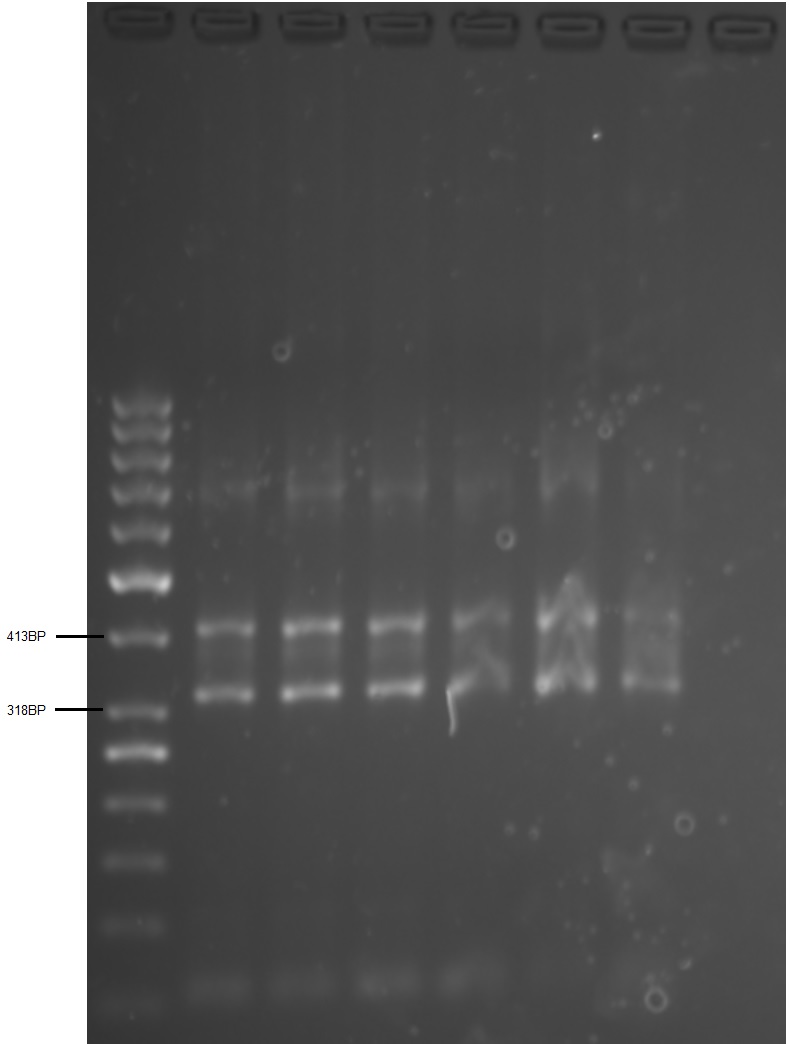
\includegraphics[width=7.29167in,height=\textheight]{./images/DNA_ACTN3-01.jpg} \hfill{}

\caption{\textbf{Figur 1}: ACTN3 R577X polymorfisme, bånd på 413bp (R)
og 318 (X) etter gelelektroforese (2\% agarose). Brønn 1 = ladder, brønn
2 og 3 = P, brønn 4 og 5 = IJ, brønn 6 og 7 = EH, brønn 8 =
H\textsubscript{2}O (ikke avbildet).}

\end{figure}

\hypertarget{diskusjon}{%
\section{\texorpdfstring{\textbf{Diskusjon}}{Diskusjon}}\label{diskusjon}}

Resultatene etter denne testen vil kunne vise hva slags genotype
testpersonene har av genet ACTN3. Dette genet er assosiert med
prestasjon i idrett. R-allelene er assosiert med prestasjon i
kraftidrett og X-allelene assosiert med prestasjon i
utholdenhetsidretter (Yang et al. 2003). Av våre fire testpersoner, fikk
tre et resultat. Alle disse har kombinasjonen RX. I følge Pickering \&
Kelly (2017) reduserer det å ha R-allelen risiko for skader. Personer
med R-allelen har ofte mer muskelmasse og høyere antall type-II
muskelfibre. Både RX og RR genotyper har en tendens til å ha økt
muskelstyrke. Yang et al. (2003) skriver i sin studie at R- og X-allelen
kan opprettholdes i populasjonen fordi begge har sine fordeler, avhengig
av miljøforhold.

Konsentrasjonen av DNA var litt lav for en av testpersonene. Dette kan
skyldes at ikke all supernatant ble fjernet i den tidlige
produksjonsfasen, eller at man ikke fikk med nok øvre fase før vi
tilsatte etanol. I den ene prøven, hvor DNA konsentrasjonen ble for lav
til videre undersøkelse, ble midtre fase forstyrret.

\hypertarget{referanser-1}{%
\section{Referanser}\label{referanser-1}}

\bookmarksetup{startatroot}

\hypertarget{deloppgave-3-vitenskapsfilosofi}{%
\chapter{Deloppgave 3:
Vitenskapsfilosofi}\label{deloppgave-3-vitenskapsfilosofi}}

1.

Popper ønsket å differensiere mellom vitenskap og pseudovitenskap. Den
tradisjonelle ideen om at vitenskap skiller seg fra pseudovitenskap ved
sin empiriske metode, hovedsakelig induktiv metode, mente han ikke var
tydelig nok. Popper mente at det fundamentale i vitenskapelig teori er
at den er falsifiserbar. Med dette menes ikke at teorien er falsk, men
at teorien har bestemte forutsigelser som kan testes og muligvis
avkreftes. En falsifiserbar teori kan altså muligvis være uriktig eller
falsk, og den er ikke kompatibel med alle mulige utfall eller
observasjoner. Popper mente at falsifisering kunne hjelpe oss å skille
vitenskapelige teorier fra pseudovitenskaplige. Vitenskapelige teorier
mente han pr definisjon er falsifiserbare, men om teorien er
falsifisert, er den usann og skal derved ikke aksepteres. Poppers
demarkasjonskriterium sier at en vitenskapelig teori er en falsifiserbar
teori, og at en uvitenskapelig teori er ufalsifiserbar. Andre
vitenskapsfilosofer er uenig i Poppers teori. Okasha påpeker at forskere
sjelden forkaster tesen selv om noen data motbeviser den. Han mener det
er nær umulig å finne en vitenskapelig teori som passer med alle data.
Det er først når mengden data som er i konflikt med teorien er
overveiende, man forkaster hypotesen. Han er også kritisk til Poppers
forestilling om at vitenskap har en «essensiell natur». Okasha løfter et
viktig spørsmål; «Er det mulig å finne et felles kriterie for hva som er
vitenskap?» Han mener også at Poppers teori har en åpenbar svakhet.
Målet ved vitenskapelig forskning er ikke alene å avkrefte teorier, men
å finne og bekrefte nye. Målet for forskere, vil derfor være å finne
støtte til egne teorier er sanne. For å gjøre det, må man til en viss
grad benytte induktiv metode.\\

Popper brukte Freud og Marx som eksempler på pseudovitenskap. Han mente
de bortforklarte alle data som ikke passet med egne teorier i stedet for
å akseptere at teoriene ikke stemte. Okasha trekker frem at Adams og
Leverrier, som begge samtidig, men hver for seg, fremmet teorien om at
det måtte finnes en ekstra gravitasjonskraft som påvirket Uranus. De
klarte å beregne seg frem til at det måtte finnes en planet til, og kort
tid senere oppdaget man Neptun. Vitenskapsmennene forkastet ikke Newtons
teori, selv om den hadde beregnet feil bane for Uranus, men klarte i
stedet å forklare svakheten i teorien. Okasha mener derfor det vil være
urett å anklage Marx for pseudovitenskap, om vi hyller Adams og
Leverrier for deres vitenskap.

I utgangspunktet mener jeg Poppers teori er god. Hvis en teori kan
falsifiseres, uten at den blir falsifisert, vil den kunne være et godt
utgangspunkt for videre studier. Problemet er at den ikke åpner for
andre usikre variabler. Det å fremme en teori som passer all data er
nærmest umulig. Vitenskaper er svært ulike, og det vil derfor være
vanskelig å finne en måte å anskue dette på. Kunnskap utvikles i en
sammenheng og må også ses i sammenheng. Jeg mener derfor Okashas tilgang
er mest riktig.

2.

Kjerne idéen i den hypotetiske-deduktive metoden er at vi bekrefter en
teori gjennom å positive svar når vi tester teoriens deduktive
konsekvenser. Man vil argumentere for en teori, i motsetning til
falsifisering, hvor man vil argumentere mot teorier. Man starter med en
teori, som enten oppstår i en «oppdagelseskontekst», hvor teorien er
oppdage eller foreslått i vitenskapene, eller i en «
begrunnelseskontekst», hvor den vitenskapelige teorien er bekreftet
eller begrunnet av data. Deretter skal man utlede de empiriske
konsekvenser fra teorien ved deduksjon. Disse konsekvensene skal så
testes gjennom observasjoner eller eksperiment. Hvis de empiriske
konsekvensene viser seg å være riktige, er teorien (induktivt) bekreftet
til en viss grad.

Eksempelvis har vi observert et sykdomsutbrudd i en populasjon. En teori
kan være at sykdommen skyldes et virus. En deduksjon fra teorien vil
være at (a) virus spres lettere enn infeksjoner av andre patogener, og
at (b) man ikke kan kurere sykdommen med antibiotika. Observasjoner og
eksperimenter viser at sykdommen både er (a) og (b). Vi har da induktivt
fått bekreftelse på at sykdommen er forårsaket av et virus.

Hempel beskriver i sin artikkel hvordan Semmelweis i Wien mellom 1844 og
1848 forsøkte å finne årsaken til en overdødelighet av barselfeber ved
en av to fødeavdelinger ved Vienna General Hospital. Semmelweis fremmet
ulike teorier som årsak til overdødeligheten. Disse avviste han
etterhvert ved å vurdere de opp mot allerede kjente fakta, eller han
gjennomførte ulike undersøkelser for å teste hypotesene. Til slutt fikk
han en idé, som viste seg å være korrekt.\\

For et deduktivt valid argument gjelder at om premissene er sanne, er
konklusjonen sann;

Om T er sann (Det vil regne når det er overskyet) , da er E (Det regner)
også sann. E er ikke sann(Det regner ikke ) T er ikke sann (Det regner
ikke når det er overskyet)

Et deduktivt usant (invalid) argument; når konklusjonen er usann, selv
om premissene er sanne:

Om T (Det vil regne når det er overskyet) er sann, da er E(Det regner)
også sann E er sann (Det regner) T er sann ( Det regner når det er
overskyet)

Et av problemene med HD metoden er at teorien handler om sannsynlighet.
Det er da ikke mulig å dedusere seg frem til en hyppighet av forekomst.
Et annet problem, er at mange andre teorier kan passe like godt med
dataene og at HD-metoden ikke tar høyde for dette.

Abduksjon forsøker å løse problemet med HD-metoden, ved at den ikke bare
krever at en teori forklarer dataen, men at den også gir bedre
forklaringer enn andre tilgjengelige teorier. I abduksjon vil den
logiske strukturen se slik ut:

En teori (T) vil gi en plausibel forklaring på våre data D1, D2.. Ingen
tilgjengelig alternativ teori vil gi like god forklaring på D1, D2.. T
er bekreftet ( til en viss grad)

En teori som forklarer flere forskjellige data og som utgår fra færre
årsaker, anses å gi en bedre forklaring.

3.

Med replikasjon menes å gjenta en undersøkelse/studie for å kontrollere
om et tidligere forskningsresultat lar seg gjenskape - om resultatene
blir de samme eller nære. De senere årene har replikasjon av tidligere
studier fått en økt interesse, fordi det har vist seg at en rekke
tidligere forskningsfunn har vært vanskelige å gjenskape. Begrepet
«replikasjonskrisen» blir benyttet til å beskrive denne utfordringen med
at foruroligende få studier lar seg replisere. Dette får betydning for
tilliten vitenskapen har. Kan man stole på de funn som blir publisert?
Innen medisin, har replikasjon stor betydning. Vi har sett at
retningslinjer for behandling baserer seg på studier som kanskje flere
år senere viser seg ikke å la seg replisere -- av ulike årsaker.
Medisinalfirmaer står bak store, kostbare studier i utviklingen av nye
medikamenter for alvorlige sykdommer som kreft og nervesykdommer. Når
disse medikamentene blir godkjent fordi de har vist seg å ha effekt,
oppstår det et krav og forventning om at disse skal gjøres tilgjengelig.
Slike nyutviklede medikamenter er svært kostbare. Ved gjennomgang av
studier innen onkologi, har det vist seg at kun 11\% av studiene var
repliserbare. Hva er årsaken til dette?

Alexander Bird fremmer base-frekvens-bias som årsak til krisen.
Base-frekvens-bias kan oppstå når man unnlater å vurdere forekomsten,
eller frekvensen av hendelsen man undersøker i populasjonen. Bird viser
at selv med en god test, vil sannsynligheten for et sant positivt svar
være lav om pre-test sannsynligheten er lav. Selv om testmetoder og
beregninger er utført korrekt, vil det være vanskelig å gjenskape de
samme resultatene. Om hypotesen har en lav sannsynlighet for å være
sann, vil man kunne få en høy andel positive resultater som i realiteten
er falsk positive (Type-I-feil) i følge Wacholder et al.~({[}2004{]}) og
Colhoun et al.~({[}2003{]}). Et eksempel på dette kan være
screeningundersøkelser for bestemte sykdommer -- som regel kreft - i en
populasjon. Selv om man har en god test, vil risikoen for å få falsk
positive være høy, om den sykdommen man screener for har en lav insidens
i populasjonsgruppen. Dette vil da kunne medføre unødvendig
sykeliggjøring og komplikasjoner.

Disse sannsynlighetene kan man beregne ved å benytte Bayes theorem;

Sannsynligheten for å ha coloncancer hvis man tester positivt på
screeningprøve (Tp) kan skrives matematisk som:

P(CC\textbar Tp)

Vi vet at:

P(CC\textbar Tp) = P(CC)P(Tp\textbar CC)

P(CC)P(Tp\textbar CC)!P (\textsubscript{CC)P(Tp\textbar{}}CC)

Frekvensen av type-I-feil og type-II-feil gir oss;

P(Tp\textbar CC) er sannsynligheten for å få falsk positivt resultat
(=0,05) og

P(Tp\textbar\textasciitilde CC) er sannsynligheten for ikke å få et
falsk negativt resultat (=0,95)

Disse verdiene gir:

P(CC\textbar Tp) = P(CC)x0,95 P(CC)x0,95!P (\textasciitilde CC)x0,05

Sannsynligheten for å ha coloncancer er (P(CC)).

Sannsynligheten for ikke å ha coloncancer (P(\textasciitilde CC) er 1 -
(P(CC)).

P(CC) er sannsynligheten for å ha coloncancer uansett hva testen viser,
og defineres som basefrekvensen av coloncanser i populasjonen.

Insidensraten av CC i Norge (2021) var 0,001.

Sannsynligheten for at man har CC gitt en positiv test vil være
P(CC\textbar Tp) = 0,001 x 0,95 0,001 x 0,95 ! 0,999x 0,05 ≈0,019 =
1,9\%

Bird trekker også frem tvilsom forskningspraksis som en del av
replikasjonskrisen, for eksempel P-hacking eller juks med data. Jevnlig
avdekkes juks i forskning. I 2010 måtte Milena Penkowa trekke seg fra
sitt professorat ved Københavns Universitet, etter at det ble avdekket
manipulering av forskningsdata helt tilbake til hennes
doktoravhandling.\\

I juli i år publiserte tidsskriftet Science en artikkel om mulig
omfattende forskningsjuks innenfor Alzheimer-forskning med utgangspunkt
i en studie publisert i tidsskriftet Nature i 2006, som Bird også
referer til i sin artikkel. Hva får forskere til å jukse? Som i andre
felt er det mye prestisje og penger som står på spill.

Lav statistisk styrke, menes også å kunne være en årsak til
replikasjonskrisen. Med statistisk styrke menes sannsynligheten for at
en test gir et resultat som gjør at man avviser en sann 0-hypotese, det
vil si sannsynligheten for ikke å få et falsk negativt svar
(Type-II-feil). Det betyr at man ikke klarer å påvise en effekt i
studiet, men som egentlig er tilstede. Dette kan også skyldes at
studieutvalget ikke var tilstrekkelig representativt for
studiepopulasjonen, eller at den statistiske styrken var for liten til å
identifisere en forskjell som statistisk signifikant. Større studier vil
være mer representative. Ved små studier vil risikoen for at
tilfeldigheter eller ukorrigerte bias påvirker resultatene være større.
Noen ganger vil det være en utfordring å skaffe nok
observasjonsgrunnlag, spesielt ved sjeldne tilstander/forekomster. Andre
ganger kan økonomi og tidspress være en faktor.

En siste ting Bird nevner som en mulig forklaring er
Publikasjons-skjevhet. Med dette menes at negative resultater ikke blir
publisert like ofte som positive resultater. Årsaken til dette kan både
skyldes at forskere ikke ønsker publikasjon, men også at tidsskrift ikke
publiserer disse data i like stor grad. Flere vitenskapsfilosofer
(Heene{[}2012{]}, Francis{[}2012{]}, Pashler og Wagenmakers{[}2012{]},
Romeo{[}2016{]}) har argumentert for dette, men Bird mener ikke dette
kan være den eneste årsak til krisen. Både forskere og tidsskriftene har
høy standard for kvalitet og har en høy terskel for statistisk
signifikans. Dette vil medføre høy sannsynlighet for at et positivt
resultat er sant. Ved teorier der det ikke foreligger annen publisert
forskning, vil man ikke vite om dette skyldes om teorien er testet med
negativt resultat, eller om teorien ikke er testet tidligere.

Alle fremsatte mulige årsaker fremstår som plausible forklaringer på
replikasjonskrisen. Som ved øvrige vitenskapsteorier, er det ikke en
sannhet. Verden er kompleks.

Litteraturliste:

Hempel, Carl G. (1966) Scientific Inquiry; Invention and Test.
\textbar{} C G Hempel, Philosophy of Natural Science (s.3-18) Princeton,
Prentice Hall.

Godfrey-Smith, P. (2003) Bayesianism and modern theories of evidence.
\textbar{} P. Godfrey-Smith, Theory and Reality: An Introduction to the
Philosophy of Science (s. 202-218) Chicago; University of Chicaago
Press.

Popper, K. (1969) Conjectures and Refutations; The Growth of Scientific
Knowledge (3. Utg) London: Routledge.

Bird, A. (2021) The British Journal for the Philosophy of Science,
vol.72, nr. 4 December 2021

Okasha S. (2016) Philosophy of Science, a very short introduction. (s.
1-70) second edition 2016, Oxford University press.

\bookmarksetup{startatroot}

\hypertarget{deloppgave-4-studiedesign}{%
\chapter{Deloppgave 4: Studiedesign}\label{deloppgave-4-studiedesign}}

Gjennom menstruasjonssyklus har kvinner i fertil alder svigninger i nivå
av kjønnshormoner. I Follikullærfasen dominerer østrogen og i
lutealfasen dominerer progesteron, selv om også østrogen har en peak da.
Det har vært reist spørsmål om disse fluktuasjoner i hormonnivåer har
inflytelse på kvinners fysiske prestasjoner. Det finnes noe forskning på
området hvor man har sett på muskelstyrke, VO2max og/eller laktat. Jeg
har tatt utgangspunkt i fem orginalartikler fra kliniske forsøk hvor man
har sett på dette.

{[}1{]}. Eur J Appl Physiol. 2003 Nov;90(5-6):505-13. doi:
10.1007/s00421-003-0889-0. Epub 2003 Jul 26. Impact of menstrual cycle
phase on the exercise status of young, sedentary women Leanne M Redman
1, Garry C Scroop, Robert J Norman

{[}2{]}. Kathmandu Univ Med J (KUMJ). 2012 Oct-Dec;10(40):25-9. doi:
10.3126/kumj.v10i4.10990. Endurance capacity and cardiorespiratory
responses in sedentary females during different phases of menstrual
cycle A Bandyopadhyay 1, R Dalui

{[}3{]}. European Journal of applied Physiology, July 7th 1994, Effects
of the menstrual cycle phase on the blood lactale responses to exercise.
m.McCracken, B. Ainsworth, A.C. Hackney

{[}4{]}. J Physiol. 1996 May 15;493 ( Pt 1)(Pt 1):267-72. doi:
10.1113/jphysiol.1996.sp021381. Changes in muscle strength, relaxation
rate and fatiguability during the human menstrual cycle R Sarwar 1, B B
Niclos, O M Rutherford

{[}5{]}. Clinical Trial J Physiol. 2001 Jan 1;530(Pt 1):161-6. doi:
10.1111/j.1469-7793.2001.0161m.x. The influence of menstrual cycle phase
on skeletal muscle contractile characteristics in humans X A Janse de
Jonge 1, C R Boot, J M Thom, P A Ruell, M W Thompson

\hypertarget{innledning}{%
\subsection{Innledning}\label{innledning}}

Den overordnede problemstillingen i de aktuelle studiene er om
hormonendringene gjennom menstruasjonssyklus har inflytelse på kvinners
fysiske prestasjon, men i de fem studiene har tilgangen vært ulik. Tre
av studiene {[}1,2 og 3{]} har hovedfokus på utholdenhet og
kardiovaskulære aspekter, og to studier {[}4 og 5{]} har undersøkt
muskelstyrke og kontraktile karakteristika.

I den første artikkelen {[}1{]} fremmes en hypotese hvor man tar
utgangspunkt i at lipider er foretrukne energikilde i lutealfase, og
forventer da en korrelert økning i fysisk prestasjon. Dette begrunnes
med at serumverdiene av østradiol {[}E2{]} og progesteron {[}P4{]} er
lave i starten av follikulærfasen og høye i lutealfasen. Begge hormoner
antas å kunne påvirke energisubstratomsetningen, termoregulering og
væske-og elektrolyttbalansen, og forfatterne har derfor en teori om at
hormonendringene vil kunne påvirke både treningskapasitet og -
prestasjon. Forfatterne viser til sprikende resultater fra tidligere
studier, og fremmer at bl.a bruk av ulike studiedesign og metoder til å
fastsette periodene i mensturasjonssyklus kan være medvirkende årsak til
dette.

Også forfatternere bak artikkel {[}2{]} viser til store sprik i
tidligere forskningsstudier og at enkelte har vist til forskjeller i
laktat-respons, vekt, plasmavolum, hb, HR og ventilasjon. De presenterer
ingen egen hypotese, men formulerer at de ønsker å evaluere fluktuasjon
i utholdenhetskapasiteten og den cardiorespiratoriske prestasjon hos
øst-indiske kvinner gjennom menstruasjonssyklus.

Forfatterne bak artikkel tre {[}3{]} ønsker å finne ut om laktat nivået
i forbindelse med intensiv løping endret seg i ML og MF fasene og de
fremmer spørsmålet om hvis dette er reelt, om man da kan benytte
laktatmålinger hos kvinnelige idrettsutøvere for å monitorere
treningsintensiteten. Forfatterne referer til studier hvor man har vist
at hvile-lipid-metabolismen og glycogenlagringen er høyere i lutealfasen
enn i follikuærfasen. Dette mener de skyldes høyere østrogen-nivå under
lutealfasen enn i follikulærfasen. Submaximal belastning, lipid
mobilisering og - oxidering virker også til å være høyere i lutealfasen.

Målet med undersøkelsen i fjerde artikkel{[}4{]} var å undersøke
effekten av fasene i menstruasjonssyklus på enkle styrketester i store
muskelgrupper, og som da har stor betydning for daglig funksjon.
Forskerne kikket også på forskjeller mellom menstruasjonsfaser og bruk
av hormonelt prevensjonsmiddel (P-pille). Dette er et interessant
spørsmål, og man kunne med fordel ha benyttet p-pillebrukere som
kontrollgruppe i flere studier. Etter menopausen hvor østrogennivået er
lavt, ses svekket muskelstyrke. Dette har fremmet hypotesen om at
østrogen påvirker skjelettmuskulatur.

Også i den femte artikkelen {[}5{]} har man undersøkt betydningen av
menstruasjonssyklus på skjelettmuskulaturens kontraktile karakteristika,
men forfatterne poengterer viktigheten av å måle hormonstatus, da dette
ikke ses gjørt i tidligere studier. Forskerne har målt muskelfunksjon
når østrogen- og progesteronverdiene var lave ( under menstruasjonen),
når østrogennåvået var høyt og progesteron lavt (sen follikulærfase) og
mens både østrogen- og progesteronnivået var høyt (lutealfasen). Dette
gir en større sikkerhet for at deltakerne er testet på det tidlspunktet
i syklus man har antatt. Forfatterne trekker frem utfordringene ved
tidligere studier, blant annet feilkilder ved måling av voluntær styrke
og usikre syklusperioder, da det ikke er tatt hormonprøver for å sikre
at man tester på riktig antatt tidspunkt i syklus. Sammenhengen mellom
mensturasjonssyklus og styrke er fortsatt uklar og de ønsker derfor å
bidra til å belyse sammenhengen bedre.

\hypertarget{teori}{%
\subsection{Teori}\label{teori}}

Man kan inndele menstruasjonssyklus i fire faser; Den tidlige
follikulære fase, som starter ved menstruasjonens første blødningsdag,
den sene follikullære fase, som strekker seg frem til eggløsning, den
tidlige luteale fase som starter ved eggløsning og den sene luteale fase
som strekker seg frem til menstruasjonens første dag.

Gjennom menstruasjonssyklus varierer serumverdiene av østradiol{[}E2{]}
og progesteron {[}P4{]}. Østradiol er lav den tidlige follikulære fase,
men stiger i den sene follikulære fase til et peak rett før egggløsning
hvor det faller brått. I den sene luteale fase har {[}E2{]} igjen en
stigning og en litt mindre peak. Progesteron er lav i hele den
follikulære fase, men stiger kraftig etter eggløsning og er høyest i den
sene luteale fase. Østrogener har en svakere proteinanabolsk effekt og
den er mer vevsspesifikk enn andosteroner. Man har likevel en antagelse
at østrogener har en anabol effekt på skjelettmuskulatur også hos
kvinner, da man ser en muskelatrofi etter overgangsalderen. Østradiol
påvirker også lipidmetabolismen.

Det kan derfor være nærliggende å tenke at de hormonelle endringene også
vil kunne ha betydning for fysiologiske parametre og fysisk prestasjon.

Både i artikkel {[}2{]} og {[}3{]} har forskerne testet deltakerne i
perioder av fasene hvor man ikke forventer en maksimal
serumkonsentrasjon av hhv østrogen og progesteon. I artikkel {[}4{]} har
man valgt å sammenligne med en kontrollgruppe som bruker p-piller, der
hormonnivåene er relativt konstante gjennom syklus. Hvis man pant en
positiv korrelasjon mellom styrke og faser i menstruasjon som man ikke
gjenfinner hos p-pillebrukere, vil dette også kunne gi viktig
informasjon om p-pillebrukere.

Teorien om at østrogen er anabol for skjelettmuskulatur, er nærliggende
da det ses en betydelig muskelsvekkelse hos kvinner etter
overgangsalderen. Vi vet at produksjon av østrogen faller gradvisgjennom
klimakteriet. Men det skjer også andre hormonelle forandringer, og vi
VET altså ikke om det er østrogen som er den ene årsaken til
muskelsvinn.

\hypertarget{metode-1}{%
\subsection{Metode}\label{metode-1}}

Metodene og designet i de fem studiene har flere likhetstrekk, men også
forskjeller. Studiedesignet i artikkel {[}1{]}, {[}2{]}, {[}3{]} og
{[}5{]} er longitudinel kohort-studie med oppfølgingstid på to sykluser
( ca 8 uker). Man følger da et utvalg - en kohort - gjennom en periode,
hvor man gjør observasjoner. Det gjennomføres ingen intervensjoner i
disse studiene. Observasjonene vil fortelle oss om det er signifikant
forskjell i de variablene vi måler på de gitte tidspunkt. Studiet bak
artikkel {[}3{]} er også randomisert, da rekkefølgen fasene de ble
testet i ble randomisert. Med randomisering menes at det gjøres et
tilfeldig utvalg. Studiedesignet i artikkel {[}4{]} er case-control,
hvor casegruppen er deltagere med normal menstruasjonssyklus og
kontrollgruppen er p-pillebrukere. Intervensjonen er da den naturlige
hormonelle fluktuasjon. Oppfølgingstiden er 8 uker. I
case-kontroll-studier følger man to (eller flere) grupper som utsettes
for ulike intervensjoner. Som regel vil case-gruppen utsettes for en
intervensjon og ikke kontrollgruppen. I dette studiet kunne man også
valgt å snu rundt og kalt p-pillegruppen intervensjonsgruppe, og
kvinnene med normal mensturasjonssyklus kontroll og da sett på
eventuelle treningsfysiologiske parametre hos kvinner som bruker
p-piller. En oppfølgingstid på to sykler forekommer noe kort. Det er
vanskelig å treffe presist ift riktig fase og hormonnivå, og ved å
utvide observasjonstiden til tre sykler, vil man få større
treffsikkerhet.

I det første studiet ble syvogtyve friske, utrente kvinner med normal
menstruasjonssyklus rekruttert gjennom annonsering. De måtte utfylle et
spørreskjema vedrørende generell og gynekologisk helse, og 16 kunne
etter dette inkluderes i studien. Deltakerne hadde normal
menstruasjonssyklus, var utrente, ikke-røykende og var ikke gravide
eller hadde brukt hormonell prevensjon de siste 6 mndr før studiens
start. En av deltakerne trakk seg pga sykdom og en deltaker ble
ekskludert pga hy VO2max som indikerte at hun ikke var utrent.
Studiestørrelsen er da relativt liten med 14 deltakere. Kohorten er en
relativt god representasjon av bakgrunnsbefolkningen, men utelukker
andelen bl.a kvinner som bruker hormonell prevensjon.

I studie {[}2{]} er 45 friske, utrente kvinner mellom 21 og 25 år fra
samme sosio-økonomiske bakgrunn utvalgt fra en post-grad avdeling ved et
universitet i India, og det fremkommer ingen opplysninger om noen ble
ekskludert. Studiestørrelsen anses som adekvat, men studiepopulasjonen
er selektert og gir ikke nødvendigvis en god representasjon av
bakgrunnspopulasjonen.

Studie {[}3{]} inkluderte 9 eumenoreiske kvinner mellom 18-32 år.
Artikkelen gir ingen informasjon om hvordan deltakerne er rekruttert,
men alle deltakere var fysisk aktive og hadde en VO2max på 46 ±2,6
ml/kg/min ved studiestart. Studiepopulasjonen er svært liten, men det er
ikke gjort styrketest.

Case-kontroll-studien i artikkel {[}4{]} rekrutterte to grupper unge,
friske, relativt utrente kvinner. Det fremkommer ingen opplysninger om
inklusjons eller eksklusjonskriterier. Den ene gruppen brukte ikke
hormonell prevensjon, og alle hadde en regelmessig menstruasjon på mlm
26 og 32 dager. Kontrollgruppen brukte en kombinasjons-p-pille, og hadde
gjort dette i minst 6 mndr. Syklus ble inndelt i tidlig- og
midt-follikulærfase, ovulasjonsfase og midt- og sen-lutealfase. I det
femte studiet {[}5{]} ble nitten friske kvinner med normal
menstruasjonssyklus rekruttert. De hadde ikke brukt hormonell prevensjon
de siste 6 mndr før studien. Deltakere med uregelmessig mensturasjon ble
eksludert, og den endelige studiepopulasjonen var 7 deltakere. Dette er
en svært liten gruppe.

I første studie {[}1{]} ble menstruasjonssyklus og eggløsning beregnet
ut fra 1. blødningsdag og eggløsningstest. Man har inndelt i
Follikuærfase (FP) og Lutealfase (LP). Det ble gjennomført fem fysiske
tester på sykkel. Først en base-line, deretter i dag 5-7 i syklus
(tidlig follikulærfase) og 21-23 (midtre/sen lutealfase) i to påfølgende
sykluser. I første syklus ble det gjennomført trinnvis test til
utmattelse, og i andre syklus ble det gjennomført en submaximal test.
Rekkefølgen av fasen testene ble gjennomført i, ble randomisert. Det ble
tappet blod før underveis og etter testing, og prøvene ble analysert for
laktat, FSH, østradiol {[}E2{]} og progesteron {[}P4{]}. VO2max, HR, VE,
VCO2, RER, RF og TV ble registrert. Dette er variabler som vil kunne gi
oss svar på spørsmålene forfatterne stiller.

I artikkel {[}2{]} benyttet man tempraturmåling for å bestemme
eggløsningstidspunkt. Testene ble gjennomført i menstruasjonssyklus dag
3 (tidlig follikulærfase) og 10 (sen follikulærfase) samt mellom dag
20-24 (lutealfase). Testene ble gjennomført flatt på på tredemølle som
en VO2max-test ( til utmattelse). I artikkelen beskrives ikke
datasettet. Resultatene presenteres i form av deskriptive variabler med
gennomsnittsverdier ±SD for preHR, BT, RR, VO2max, max. minuttvolum,
O2puls, utholdenhetskapasitet og maxHR.

Testene i studie {[}3{]} ble gjennomført på tredemølle i syklusdag 6-9
(Midtfollikulærfase) og 6-9 dager etter ovalusjon (Midtlutealfase).
Eggløsning ble stadfestet ved temeraturmålinger, samt hormonanalyse av
morgenurin på testdag. Rekkefølgen på fasene det ble gjennomført test,
ble randomisert. Testene som ble gjennomført var en gradvis økning av
belastning i 30 min. Etter 30 min, ble belastningen økt til 90\% av
VO2max og deltakerne løp til utmattelse. Blodprøvene ble tatt rett før
test, og 3 og 30 minutter etter test.

I det første styrkestudiet {[}4{]} ble deltakerne testet ukentlig
gjennom to fulle sykluser. Begge ben ble testet hver gang, og
gjennomsnitt beregnet. Syklus ble beregnet tilbake fra siste
menstruasjons første dag (SM) og ovulasjon beregnet 14 dager før dette.
EF = 1-7d, MF = 7-12d, MC = 12-18d, ML = 18-21d og LL = 21-32d. Den
maximale voluntære isometriske styrke av quadriceps ble testet. De
kontraktile delene av quadriceps ble stimulert og man beregnet
relaxasjonstiden. For å se på trettbarheten, ble muskelen igjen
stimulert og Trettbarhets index ble målt som den prosentvise mistede
kraft over 3 minutter. Håndgrepskraft ble også målt med et
hånd-dynamometer. Variablene i studiet er menstruasjonssyklus-periodene
og muskelstyrke i quadriceps og håndgrep, og trettbarhet og
relaxasjonsevne i quadriceps.

I det siste studiet {[}5{]} målte man muskelstyrke, trettbarhet og
kontraktilitet i de ulike fasene av syklus. Man inndelte fasene i
blødningsfase, sen follikulærfase og lutealfase. Testing i sen
follikulærfase er vanskelig å time, da peak i østrogennivå kun varer ca
3 dager. Man valgte derfor å teste to dager i denne fasen, for å øke
treffsikkerheten. Testen som ble gjennomført den dagen hvor det ble målt
høyest østrogen og lavest progesteron ble benyttet. Man gjennomførte
isometrisk test og trettbarhetstest av quadriceps før isokinetisk
knefleksjon og -ekstensjon styrke og trettbarhet. Deretter gjennomførte
man håndgrep-test. Det ble benyttet temperaturmåling for å finne
ovulasjonsdag, og deltakerne fylte ut spørreskjema om symptomer. Før
hver test, ble det tatt blodprøver, som ble analysert mhp FSH, LH,
østrogen og progesteron.

\hypertarget{statistisk-analyse}{%
\subsection{Statistisk analyse}\label{statistisk-analyse}}

Forfatterne i den første artikkelen {[}1{]} benyttet lineære
regresjonsmodeller i analysen av datasettet. I den statistiske analysen
ble det benyttet en Student´s parret t-test og analysa av varians
(ANOVA) for å bestemme forskjellen mellom follikullær- og luteal-fase og
pre- og post-test treningsdata. For å sammenligne det
cardiorespiratoriske og p-laktat responset på hhv VO2 max-test og
laktatprofiltest, ble det benyttet en RMANOVA. Også i andre artikkel
{[}2{]} benyttet man ANOVA for å sammenligne forskjellen i
gjennomsnittet som er observert i de ulike menstruasjonsfasene, men i
tredje artikkel {[}3{]} ble data statistisk analysesert ved en Friedman
analyse av variance og Fisher post-hoc testing av den gjennomsnittlige
forskjellen. I artikkel fire {[}4{]} ble det benyttet ANOVA for å
sammenligne syklusfasene, og disse ble testet ved Student´s parret
t-test. Student´s uparrede t-test ble benyttet for å sammenlgne de to
gruppene ANOVA ble også benyttet i artikkel fem {[}5{]} for å se
forskjeller i hormonverdier og styrketester.

\hypertarget{resultater-2}{%
\subsection{Resultater}\label{resultater-2}}

Det er noe sprikende resultataer i de fem artiklene, men studiene er
designet noe ulikt, og variablene er ikke de samme.

Studiet bak artikkel {[}1{]} målte hormonprofil i hvile. Denne viser at
basal {[}E2{]} og {[}P4{]} var høyere i LP enn i FP. Dette er ikke
uventet, da test i FP ligger i tidlig follikullærfase, hvor man også
forventer at {[}E2{]} er lav. LH var lav i begge faser (av samme årsak).
Under aktivitet over 75\% av VO2 max så man en signifikant stigning i
{[}E2{]} i LP. Etter aktivitet økte {[}E2{]} i begge faser. Man fant
ingen forskjell i peak power output, tid til utmattelse eller totalt
arbeid mellom de to fasene. Det ble påvist signifikant
interaksjonseffekt mellom fase (LP) og treningsbelastning (\%WLmax). Man
så ingen endring i ventilasjon, RF, HR, men CO2 output og var lavere i
LP og ved høy intensitet så man lavere RER i LP. Det ble påvist en
positiv korrelasjon mellom basal {[}E2{]} og RER i FP.
Laktat-konsentrasjonen var lavere ved alle intensitetetr i LP. Under høy
intensitet var s-laktat signifikant høyere ved 15m, 20 m og post i FP.

I artikkel {[}2{]} fant man en signifikant lavere pre-HR i
blødningsfasen (tidlig FP) enn i sen FP og LP. Forfatterne fant også at
VO2max, O2puls, max MV og utholdenhetskapasitet var signifikant lavere i
follikulærfasen.

I det tredie studiet {[}3{]}, hvor det fokuseres på laktat, ser man at
løpstid til utmattelse var lik i begge faser, og at hvile-laktatverdiene
også var like. Post-laktatverdiene var sigifikant lavere i ML enn i MF
både etter 3 og 30 minutter.

Studien i artikkel {[}4{]} viser ulike resultater for de to gruppene.
Quadriceps styrke; i case- gruppen så man en topp i MC, og det var
signifikant større styrke da enn i alle andre faser. For kontrollgruppen
(p-pille), var det ingen signifikant endring mellom fasene. Man så at
kontrollgruppen generelt var svakere enn case-gruppen, men mener dette
skyldes en lavere kroppsvekt i denne gruppen. Håndgrep styrke; var også
signifikant større i MC sammenlignet med alle andre faser i
case-gruppen. Også her var kontrollgruppen svakere enn case-gruppen.
Både quadriceps styrke og håndgrepsstyrke var lavest i LL. Quadriceps
kontraktile egenskaper: Relaxasjonstiden var langsomst i MC i
case-gruppen. Det ble funnet signifikante forskjeller mellom MC og EF,ML
og LL. I kontrollgruppen fant man ingen signifikante forskjeller.
Quadriceps fatigue index: I case-gruppen, var muskelen mer trettbar i
MC, enn i de andre fasene, og signifikant forskjell til LL. Hos
kontrollgruppen fant man ingen signifikant forskjell.

Dette står i kontrast til det siste studiet {[}5{]} hvor man ikke fant
signifikant forskjell i styrke verken i quadriceps, for kneflexorer
eller extensorer eller ved håndgrep. Man fant hormonverdier som endret
seg som forventet gjennom syklus hos individene.

\hypertarget{diskusjon-1}{%
\subsection{Diskusjon}\label{diskusjon-1}}

Konklusjonen i artikkel {[}1{]} er at treningskapasitet (VO2max og
laktatterskel) ikke er påvirket av menstruasjonssyklus hos unge utrente
kvinner. Under submax. belastning i LP ser man et metabolsk respons
tolket som en økt utnyttelse av lipider son energikilde. Forfatterne
viser til tidligere forsøk som har vist det samme, men at en del studier
ikke har fokusert på metabolisme, men kun studert fysiologiske
endepunkt. De mener derfor at metabolsk respons, som relativ
treningsintensitet (\% VO2max eller \% WLmax), er essensiell for å kunne
oppnå dypere forståelse af fyiologisk respons på vedvarende trening med
ulik intensitet hos kvinner i fertil alder.

Forfatterne mener studeiet viser at det er behov for mer forskning på
området. De påpeker at den store variabiliteten i hormoner både inter-
og intrasubjekt skaper vansker med å oversette resultatene - spesielt
når det er benyttet små kohorter. De foreslår å benytte oral hormonell
prevensjon, som vi gi en-fase hormoner utenom mensturasjon, og vil være
enklere for forskere å forholde seg til.

I artikkel {[}2{]} finner jeg diskrepans i artiklens resultater og
konklusjon. I resultatene sine, beskriver forfatterene at pre-HR var
lavere i tidlig FP enn i sen FP og LP, men i diskusjonen skriver de at
det er en forhøyet preHR i LP. Dette forklarer de med økt
sympatikusaktivitet, men BT er stabilt gjennom alle faser, og man vil
også forvente et økt BT ved økt sympatikusaktivitet. Forfatterne skriver
også i konklusjonen at de ikke finner signifikant forskjell på VO2max,
O2puls, max MV, utholdenhetskapasitet og max HR, men i resultatene
skriver de at disse parametrene var signifikant lavere i FP.

Funnene i artikkel {[}3{]} tyder på en endret respons på blodlaktat i de
ulike menstruasjonsfasene, som også andre forskere har funnet. Det er
også forskere som har rapportet ingen signifkante forskjeller i de ulike
fasene. Forfatterne fremmer da ulike muligheter for bias i disse
studiene.

Forfatterne konkluderte i artikkel {[}4{]} at funnene viste at musklene
hadde størst styrke, var langsommere og mer trettbare midtsyklisk hos
kvinner med normal mensturasjonssyklus. Man fant ikke lignende
forskjeller hos kvinner som benyttet hormonell oral prevensjon.
Østrogennivået er høyest rett før eggløsning, og det er foreslått som
mulig årsak. I muskelcellene finnes også testosteronreseptorer, og da
testosteron også øker i samme periode, dette kunne være den
tilgrunnliggende årsak. Forfatterne har testet kontraktilitet hos unge
menn og sammenlignet disse resultatene med kvinnenes og kun funnet
endring i midtsyklus. Dette mener de peker mot at det ikke er
testosteron som er årsak til endringen. Østrogen har en høy
serumkonsentrasjon også i lutealfase. Man burde derfor funnet de samme
resutater i LL. Forfatterne fremmer at det i LL også er høye nivåer av
progesteron, og at en mulig årsak er at progesteron kan inhibere
effekten av østrogen. Hos postmenopausale kvinner, hvor styrken er lav
ift muskelmasse, er også progesteronnivået lavt, hvilket ikke støtter
denne teorien. Temperaturendringen i cyklus anser forfatterne som ikke
mulig årsak til relaxasjonsresultatene, da musklene var raskest i LL og
EF hvor kroppstemperaturen er høyere enn i MF og MC.At man ikke fant
forskjeller gjennom syklus hos kontrollgruppen (P-piller), mener
forfatterne skyldes at serumverdiene av progesteron og østrogen er
stabile gjennom pillefasen.

Forfatterne av artikkel {[}5{]} sammenligner sine funn med artikkel
{[}4{]} hvor funnene var signifikante. De forklarer dette med en
dårligere definert midtsyklus-periode i {[}4{]}, og at hormonnivåene
derfor kan ha fluktuert signifikant. De fremmer derfor viktigheten i å
måle hormoner testdag for å kunne dokumentere fase. Dette er viktig når
man skal vurdere testresultataer opp mot syklus.

\hypertarget{konklusjon-1}{%
\subsection{Konklusjon}\label{konklusjon-1}}

Studiene bak artiklene har noe ulik tilgang til det mer generelle
spørsmålet; påvirker den hormonelle endring i kvinners
menstruasjonssyklus fysiske prestasjoner? Det fremstår klart at det er
særdeles viktig å kartlegge eksakt hvor i syklus kvinnene er, hvis man
skal kunne trekke konklusjoner om hormonendringene har signifikant
betydning. Den sikreste måten å gjøre dette på, er blodprøver på
testdag. Syklus bør inndeles i tidlig og sen follikulærfase og tidlig og
sen lutealfase. Det er i sen follikulærfase østrogen har sitt største
``peak'' og i tidlig lutealfase progesteron ``peaker''. Da har også
østrogen en mindre peak, men denne er betydelig lavere enn i sen
follikulærfase.

Som alle artikler konkluderer med; det er behov for flere studier for å
kunne besvare spørsmålet.

\bookmarksetup{startatroot}

\hypertarget{deloppgave-5-analysere-repeterte-muxe5linger}{%
\chapter{Deloppgave 5: Analysere repeterte
målinger}\label{deloppgave-5-analysere-repeterte-muxe5linger}}

\bookmarksetup{startatroot}

\hypertarget{reeranser-deloppgave-3}{%
\chapter{Reeranser Deloppgave 3}\label{reeranser-deloppgave-3}}

::: \{\#refs\}

::: Tanner, R. K., and C. J. Gore. 2012. Physiological Tests for Elite
Athletes 2nd Edition. Book. Human Kinetics.
https://books.google.no/books?id=0OPIiMks58MC

::: Hempel, Carl G. (1966) Scientific Inquiry; Invention and Test.
\textbar{} C G Hempel, Philosophy of Natural Science (s.3-18) Princeton,
Prentice Hall.

::: Godfrey-Smith, P. (2003) Bayesianism and modern theories of
evidence. \textbar{} P.

::: Godfrey-Smith, Theory and Reality: An Introduction to the Philosophy
of Science (s. 202-218) Chicago; University of Chicaago Press.

::: Popper, K. (1969) Conjectures and Refutations; The Growth of
Scientific Knowledge (3. Utg) London: Routledge.

::: Bird, A. (2021) The British Journal for the Philosophy of Science,
vol.72, nr. 4 December 2021

::: Okasha S. (2016) Philosophy of Science, a very short introduction.
(s. 1-70) second edition 2016, Oxford University press.

:::{[}1{]} Eur J Appl Physiol. 2003 Nov;90(5-6):505-13. doi:
10.1007/s00421-003-0889-0. Epub 2003 Jul 26. Impact of menstrual cycle
phase on the exercise status of young, sedentary women Leanne M Redman
1, Garry C Scroop, Robert J Norman

:::{[}2{]} Kathmandu Univ Med J (KUMJ). 2012 Oct-Dec;10(40):25-9. doi:
10.3126/kumj.v10i4.10990. Endurance capacity and cardiorespiratory
responses in sedentary females during different phases of menstrual
cycle A Bandyopadhyay 1, R Dalui

:::{[}3{]} European Journal of applied Physiology, July 7th 1994,
Effects of the menstrual cycle phase on the blood lactale responses to
exercise. m.McCracken, B. Ainsworth, A.C. Hackney

:::{[}4{]} J Physiol. 1996 May 15;493 ( Pt 1)(Pt 1):267-72. doi:
10.1113/jphysiol.1996.sp021381. Changes in muscle strength, relaxation
rate and fatiguability during the human menstrual cycle R Sarwar 1, B B
Niclos, O M Rutherford

:::{[}5{]} Clinical Trial J Physiol. 2001 Jan 1;530(Pt 1):161-6. doi:
10.1111/j.1469-7793.2001.0161m.x. The influence of menstrual cycle phase
on skeletal muscle contractile characteristics in humans X A Janse de
Jonge 1, C R Boot, J M Thom, P A Ruell, M W Thompson

:::{[}6{]} Browner, Newman: Designing clinical Research, 5th edition,
Wolters Kluwer, ISBN-13.978-1-975174-40-8

:::{[}7{]} https://psyarxiv.com/p39sc/ QALMRI- method

\hypertarget{refs}{}
\begin{CSLReferences}{1}{0}
\leavevmode\vadjust pre{\hypertarget{ref-bartlett2003}{}}%
Bartlett, John M. S., and David Stirling. 2003. \emph{PCR Protocols}.
Methods in Molecular Biology. Humana Totowa, NJ.
\url{https://link.springer.com/book/10.1385/1592593844}.

\leavevmode\vadjust pre{\hypertarget{ref-eynon2012}{}}%
Eynon, Nir, Jonatan R. Ruiz, Pedro Femia, Vladimir P. Pushkarev, Pawel
Cieszczyk, Agnieszka Maciejewska-Karlowska, Marek Sawczuk, et al. 2012.
{``The ACTN3 R577X Polymorphism Across Three Groups of Elite Male
European Athletes.''} Edited by Nuria Garatachea. \emph{PLoS ONE} 7 (8):
e43132. \url{https://doi.org/10.1371/journal.pone.0043132}.

\leavevmode\vadjust pre{\hypertarget{ref-halperin2015}{}}%
Halperin, Israel, David B. Pyne, and David T. Martin. 2015. {``Threats
to Internal Validity in Exercise Science: A Review of Overlooked
Confounding Variables.''} \emph{International Journal of Sports
Physiology and Performance} 10 (7): 823--29.
\url{https://doi.org/10.1123/ijspp.2014-0566}.

\leavevmode\vadjust pre{\hypertarget{ref-hopkins2000}{}}%
Hopkins, Will G. 2000. {``Measures of Reliability in Sports Medicine and
Science.''} \emph{Sports Medicine} 30 (1): 1--15.
\url{https://doi.org/10.2165/00007256-200030010-00001}.

\leavevmode\vadjust pre{\hypertarget{ref-pickering2017}{}}%
Pickering, Craig, and John Kiely. 2017. {``ACTN3: More Than Just a Gene
for Speed.''} \emph{Frontiers in Physiology} 8 (December): 1080.
\url{https://doi.org/10.3389/fphys.2017.01080}.

\leavevmode\vadjust pre{\hypertarget{ref-schadock2015}{}}%
Schadock, Ines, Augusto Schneider, Elton Dias Silva, Marcia Rubia Duarte
Buchweitz, Marcio Nunes Correa, Joao Bosco Pesquero, Edgar Julian
Paredes-Gamero, Ronaldo Carvalho Araujo, and Carlos Castilho Barros.
2015. {``Simple Method to Genotype the ACTN3 R577x Polymorphism.''}
\emph{Genetic Testing and Molecular Biomarkers} 19 (5): 253--57.
\url{https://doi.org/10.1089/gtmb.2014.0299}.

\leavevmode\vadjust pre{\hypertarget{ref-yang2003}{}}%
Yang, Nan, Daniel G. MacArthur, Jason P. Gulbin, Allan G. Hahn, Alan H.
Beggs, Simon Easteal, and Kathryn North. 2003. {``ACTN3 Genotype Is
Associated with Human Elite Athletic Performance.''} \emph{The American
Journal of Human Genetics} 73 (3): 627--31.
\url{https://doi.org/10.1086/377590}.

\end{CSLReferences}



\end{document}
